% CVPR 2022 Paper Template
% based on the CVPR template provided by Ming-Ming Cheng (https://github.com/MCG-NKU/CVPR_Template)
% modified and extended by Stefan Roth (stefan.roth@NOSPAMtu-darmstadt.de)

\documentclass[10pt,twocolumn,letterpaper]{article}

%%%%%%%%% PAPER TYPE  - PLEASE UPDATE FOR FINAL VERSION
%\usepackage[review]{cvpr}      % To produce the REVIEW version
\usepackage{cvpr}              % To produce the CAMERA-READY version
%\usepackage[pagenumbers]{cvpr} % To force page numbers, e.g. for an arXiv version

% Include other packages here, before hyperref.
\usepackage{graphicx}
\usepackage{amsmath}
\usepackage{amssymb}
\usepackage{booktabs}


% It is strongly recommended to use hyperref, especially for the review version.
% hyperref with option pagebackref eases the reviewers' job.
% Please disable hyperref *only* if you encounter grave issues, e.g. with the
% file validation for the camera-ready version.
%
% If you comment hyperref and then uncomment it, you should delete
% ReviewTempalte.aux before re-running LaTeX.
% (Or just hit 'q' on the first LaTeX run, let it finish, and you
%  should be clear).
\usepackage[pagebackref,breaklinks,colorlinks]{hyperref}


% Support for easy cross-referencing
\usepackage[capitalize]{cleveref}
\crefname{section}{Sec.}{Secs.}
\Crefname{section}{Section}{Sections}
\Crefname{table}{Table}{Tables}
\crefname{table}{Tab.}{Tabs.}


%%%%%%%%% PAPER ID  - PLEASE UPDATE
\def\cvprPaperID{101} % *** Enter the CVPR Paper ID here
\def\confName{CVPR}
\def\confYear{2024}


\begin{document}

%%%%%%%%% TITLE - PLEASE UPDATE
\title{Beyond Lip Reading - Inferring Voice Qualities from Visual Data}

\author{John Wood, 
Columbia University
{\tt\small john.wood@columbia.edu}
\and Jacob Wahbeh,
Columbia University
{\tt\small jacob.wahbeh@columbia.edu}
}
\maketitle

%%%%%%%%% ABSTRACT
\begin{abstract}
   Whereas there have been many successful and well-studied methodologies, symbolic representations, and processes for recovering a speaker's words from video / visual-only data, the reproductions of voice have been lacking in reproducing qualities of voice such as pitch, intensity, shimmer, jitter, and harmonics. We have worked towards building a corpus and model to attempt to recover these quantitatively derived qualities from the visual data, to see which ones can be recovered or not. Unfortunately, we were unable to produce any models effective at predicting these qualities of voice despite a variety of attempts.
\end{abstract}

%%%%%%%%% BODY TEXT
\section{Introduction}
\label{sec:intro}

There have been no shortages of papers and processes for distilling spoken words from visual-only data sources, i.e. performing lip reading. Fenghour \etal 2021 \cite{Fenghour2021} does a thorough job reviewing the corpora, pre-processing techniques, neural network architectures, and results of these processes. Ultimately, the target goal is to produce understandable words / sentences for human consumption. However, there are many other complexities to human vocal communication which these methods are not trained to reproduce. As a simple example, a rising pitch can suggest if the speaker is posing the statement as a question or topic of discussion versus a fact. After all, as we speak, the qualities of our voice modulate due to changes in emotional state and as we purposefully modulate our voice to convey meaning and context such as excitement, boredom, sarcasm, amongst other information. Therefore, to attempt to recover these vocal qualities to fully represent the intent of the speaker from visual only data, we have worked to build a set of models to predict the pitch, intensity, harmonics, jitter, and shimmer from video-only data.

NB: Code available at \href{https://drive.google.com/file/d/1mdd65EOMFP_0xZQxeuzi8KavXK4nI_mL/view?usp=drive_link}{link}

%-------------------------------------------------------------------------
\subsection{Motivating Findings}

The work that motivated our initial interest in this particular problem is our observations of attempts to  recreate voice from video data. For instance, while RobustL2S by Sahipjohn \etal 2023 \cite{RobustL2S} does a remarkable job at inferring the words of the speakers with lip reading alone, the pitch and intensity of speaking in the resulting audio recreations can vary from the original data. For independent examination of their results, Sahipjohn \etal 2023 have provided a stellar website presenting their work, which includes examples of the aforementioned phenomenon of acoustic deviances: \href{https://neha-sherin.github.io/RobustL2S/}{https://neha-sherin.github.io/RobustL2S/}.

The goal of this paper is to create an experiment to tease out the quantitatively observable elements of speech and see their relative predictability, both independent and in comparison to a baseline prediction about a speaker's median vocal qualities.  

%------------------------------------------------------------------------
\section{Related Work}
\label{sec:related}

There is a lot of related work across multiple disciplines including prior work involving lip reading automation, emotion detection automation, voice to image generation, and video to voice generation, that culminated in the means for and hypothesis that we could predict the auditory qualities of speech from video-only input.

%-------------------------------------------------------------------------

\subsection{Auditory and Visual Emotion Detection Automation}

One of the elements that forms the basis of our hypothesis that vocal traits can be recovered from visual information is the twofold existence of evidence that emotion can be recovered from visual information and that emotion can / does result in changes in vocal qualities versus the baseline. The relevance of both audio and video information to predicting emotion is discussed thoroughly in Zhicheng \etal 2023 \cite{EmotVid2023}, where independently, video and audio are shown to be predictive of emotion. Together, they are shown to be even more efficacious. Reinforcing the vocal quality side of the equation, Saini \etal 2023\cite{EmotPitch2023} discusses the relationship in more detail about how pitch and intensity, amongst other vocal cues, can be fundamental to recovering emotion.

The logical through-line is that there's some function \(f(x)\) which maps pixels to emotion and some function \(g(x)\) which maps emotion to deviations in baseline vocal qualities. Thus, we imagine there is some differentiable function, \(g(f(x))\), which could map pixels to deviations in baseline vocal qualities.

\subsection{Voice to Image Generation}

Speech2Face by Oh \etal 2019\cite{Speech2face} suggests a useful predictive correlation between one's appearance and one's vocal qualities. The finding here is that the researchers were able to use a sound file to generate an image of a person's face, and for that generated image to have some vague correspondence to a person's actual face. If this model is producing a function, f(x), we aspire to its' inverse, \(f^{-1} (x)\) to use video to generate sound.

On a philosophical note, we are hesitant to proliferate models and methodologies which (potentially / likely) use individuals' protected physical characteristics to create inferences. It is in this spirit that, while our expectation for our resultant work to find some success in predicting the median speaker qualities based on image / video alone, we intend to concentrate on judging the efficacy of the model on its relative predictions of rising and falling vocal qualities, not on absolute resulting values.

\subsection{Lip Reading Automation}

At the time of writing, we feel confident that lip reading automation is a solved problem. While there are many approaches and methodologies (mentioned earlier in Fenghour \etal 2021 \cite{Fenghour2021}) , we find the viseme to be the most compelling fundamental building block (either explicitly or implicitly extracted) from which models can be built. Explored more thoroughly in Fenghour \etal 2023\cite{Fenghour2023}, visemes are the clusters of facial movements which occur when making a particular vocalization / set of vocalizations. For instance, as noted in Jachimski \etal 2017 \cite{Elephant2017} , "elephant juice" and "I love you" involve the same fundamental lip movements, in the same order, to produce. Once the building blocks are gathered, then it is then incumbent on using an LLM or equivalent to weight the relative probabilities of the various potential constructions using the visemes to ultimately provide the most likely words / sentences spoken. Another approach, taking some inspiration directly from the construction of LLMs, is AV-HuBERT by Shi \etal 2022 \cite{AVHuBert}. The fundamental idea here is that one utilizes a hybrid ResNet and Transformer architecture to succeed on a self-supervised fill-in-the-blank tasks on video, resulting in both useful embeddings as well as success at performing lip reading. Due to the efficacy of existing models and methodologies, we felt confident in not pursuing marginal improvements for this particular problem.

\subsection{Existing Video Corpora}

Before embarking on establishing our own corpus, we performed a brief survey of existing corpora which could have met our needs. Popular corpora for the task include GRID-4S, TCD-TIMIT-3S, Lip2Wav, LRS2, and more recently, LSR3, each certainly worth their HDD capacity in gold. However, each has their specific drawbacks for our use cases. Lip2Wav by Prajwal \etal 2020\cite{LipWavCorpus2020}, for instance, is limited to a handful of speakers, 5, of which are lecturing and therefore unlikely to generate emotions besides bouts of enthusiasm for particular topics.  LRS2 by Son Chung \etal 2017\cite{LipCorpus2017}, with over 800 citations and over 90 papers utilizing the dataset, has only short-form utterances and is professionally produced, likely resulting in a consistency of demeanor and other controllable audio qualities. LRS3, by Afouras \etal 2018\cite{LSR3} has over 400 hours of TED Talk data from over 5500 speakers, which in theory could support our efforts, supposing some metadata to align speakers across the thousands of smaller clips. However, at the time of writing, the robots.ox.ac.uk site for Lip Reading Datasets did not have LSR3 available for download. 

%------------------------------------------------------------------------
\section{Methodology}
\label{sec:methodology}

Our methodology for performing this research was extensive due to the nature of the problem - specifically, we needed a corpus that would represent both a speaker's baseline audio characteristics (pitch / intensity / harmonics / etc.) as well as their audio characteristics when they deviate from that baseline. 

To achieve this, we developed our own corpus based on long-form conversations conducted in a semi-consistent environment. The long-form nature of the source datasets would facilitate 1) having enough data for an individual speaker to infer a baseline and 2) provide ample time (and stimulation) for the conversation to inspire a diversity of emotions that would cause the speaker to deviate from their baseline speaking qualities. We then collected the necessary metadata from the models using standard speech analysis tooling and libraries to create the speaker diarization and ultimately the audio metadata. 

We then purposefully avoided a common processing step in lip-reading models (for instance, used by Sahipjohn \etal \cite{RobustL2S} )  which is to use a Lip Encoder, i.e. a model which will remove excess visual data and zero in on the lips itself. We purposefully removed this to allow for the capture of other information that may be predictive of these other audio qualities. For instance, the distance between a speaker and the microphone may be conducive to predict intensity of speech. Alternatively, the upward movement of the eyebrows relative to the eyes may be predictive of a raised pitch, as the entirety of the facial expression may express surprise or the onset of a questioning mood.   
%-------------------------------------------------------------------------

\begin{figure}[t]
  \fbox{ 
   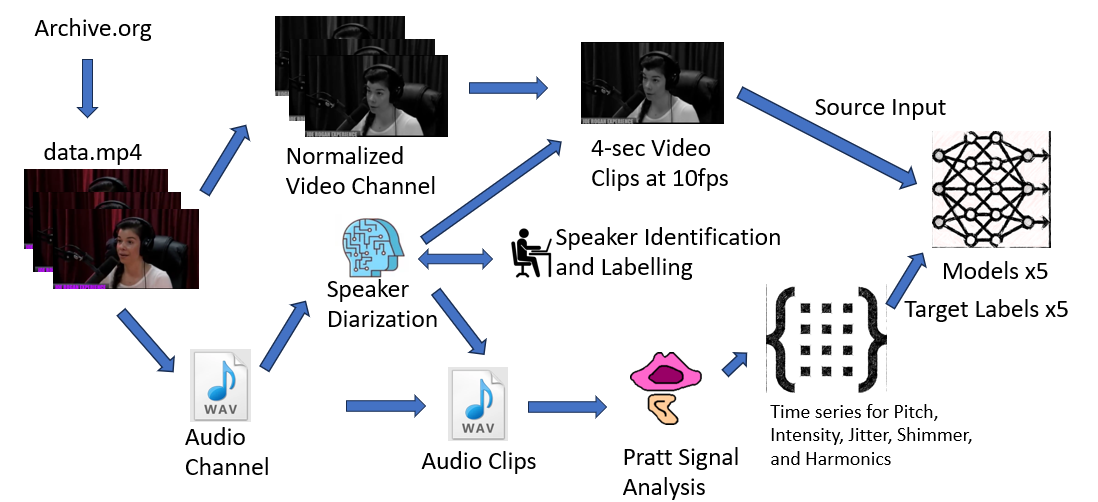
\includegraphics[width=0.9\linewidth,left]{Process Flow.png}
   }
   \caption{Data processing pipeline}
   \label{fig:onecol}
\end{figure}

\subsection{Data Collection}

As our "dynamic" data set, we chose the "Joe Rogan Experience Podcast", available as MP4 audio / video files on archive.org. We chose this due to the numeracy of the episodes, the diversity of speakers, the length of each episode (with many eclipsing 2 hours), and the dynamism of the host, Joe Rogan. We pulled select episodes from 200 to 600, limited to episodes with 1 guest which did not span multiple episodes, and also removed conversations where the speaker was not visible speaking, as was the case the the John McAfee episode. 

To note, we are aware that the population of individuals appearing on the JRE podcast, while being inclusive of entertainers, political personalities, and academics (more often than not in the exercise science and health sciences)  from California and Texas, is not generally inclusive of people across different groups / populations / economic strata / cultural backgrounds (although there is some representation across some races,  genders, and ages). However, the time horizon to, at scale, find more ideal long-form datasets unfortunately was not supported. Out goal here, though, was not to provide a tool for general consumption or use, but to test the feasibility of extracting speaker qualities from video-only input. To our credit, though, the other long-form dataset that is popular, Lip2Wav\cite{LipWavCorpus2020}, only employs 5 speakers, 3 of whom are white men and 2 which are southeast Asian men.

\subsection{Data Processing}

Once we had the mp4 files, we extracted the video and audio into separate files. For the audio files, we performed speaker diarization (i.e. split the audio file into segments by the speaker) using the pyannote.audio library\cite{Bredin23}. We then fed these segmented audio files into a Pratt\cite{Pratt}-based library called parselmouth\cite{Parselmouth}.  Parselmouth is a convenient python-based tool we used to extract the voice qualities we were looking for, in 0.1 second intervals, which would become the basis for the data points our model would attempt to predict. We also accumulated this data to create speaker median values, which we would predict in tandem with the temporally-associated values. Out hope was that even if the model fails to correctly predict the median values, we could see predictions that were correctly above or below the median when relevant. 

For our target labels, we chose pitch, intensity, shimmer, jitter, and harmonics. Pitch, or tone, is the rate of vibrations of a sound. Intensity, or loudness, is the physical magnitude or power of a sound wave. Shimmer is a measure of instability of vocal cord vibrations. Jitter is the .Harmonics, or harmonics to noise ratio, is ,to quote Fernandes \etal 2018\cite{Harmon2018}, the ratio between periodic and non-periodic components of speech sound. To put it in layman's terms, it's the additive noise that your vocal chords might produce due to aging or disease, amongst other factors.

For our video-only source data, we used the moviepy python library to remove the audio, resize the video down to 640x360 resolution, turn this images to greyscale, and to down-sample to 10 frames per second. 

Furthermore, we also created a separate video-only source data using cv2's Haar Cascade for facial recognition, introduced in Viola 2001\cite{HaarCascade2001}.

\subsection{Model Construction}

We created a plurality of different model architectures, with our original model consisting of 3 sets of 3D convolutions, and 3 linear layers. Furthermore, each convolutional layer featured a post-convolution BatchNorm, LeakyReLu, and MaxPool. We, in particular, sought out the 3D convolutional neural networks, first introduced by Ji \etal 2012 \cite{Ji3DConv}, as we intended to use video data with a temporal dimension and wanted our convolutions to have the opportunity to seek patterns over length, width, and time.  

However, as our model training continuously converged onto producing a constant output irrelevant of the input video frames, we tried a series of changes including tweaking the hyper-parameters, changing the activation functions,  reducing layers, scaling the inputs and outputs, and even removing convolutional layers altogether and using stacks of linear layers. 

\subsection{Model Evaluation}

There were a few different modalities that we planned to test the hypothesis that we could predict the audio qualities. The first would be a simple observation that the model was training by the loss decreasing over time and being able to extract an accuracy from the train and test sets. The second planned evaluation would be a correlation and r squared between the median value (the first item predicted in the target output) and the actual median for a speaker. While we were not as interested in this result, prior work suggested the possibility of achieving some accuracy. Finally, we also took the slope of the labels as well as the predicted labels and took a correlation and r squared of the two. This was the indicator we were most excited for, as it would show that, irrelevant of the absolute values predicted, that we could predict the relative ups and downs of a speaker's speech based on the video-only input.

%------------------------------------------------------------------------
\section{Experimental Results}
\label{sec:results}
%-------------------------------------------------------------------------

We ran 5 different experiments for each of the key audio qualities of voice, passing the entirety of . Furthermore, we ran and re-ran the pitch experiment with multiple variations of the model (described earlier) in an attempt to potentially get any predictability out of the model. Finally, we also filtered the data down to the face-only pixels to attempt to reduce the computations per epoch and increase the epochs into the 100s. Unfortunately, in all cases, the model outputs converged towards producing constant output independent of the input frames / pixels. This was suggestive to us of the input video data being insufficiently predictive, given that the Bayes Optimal Classifier will consistently predict the mean of a dataset, i.e. the expected value of the prior probability times the values, if the input data i.e. the probability of event B is independent of the probability of A.

This was a highly surprising result for us. At the very least, we expected that there would be some, potentially unfortunate but viable route that the model might take to discriminate between our video input to develop its outputs. For instance, one (unfortunate but biologically sound) methodology to create two potential internal representations to then use in predictions for pitch might be for the model to discern male from female speakers. On average, male speakers have pitches between 85 to 155Hz, whereas female speakers have pitches between 165 to 255Hz\cite{Fitch1970}. In theory, if the model were to learn to differentiate males from females on the podcast, then it might be able to make a differentiated prediction.

In contrast, we will admit that we were not extremely confident that we would find a pattern for vocal intensity, so the lack of a performing model is not too surprising. This is because post-processing specifically targeting normalizing the intensity of sound from a speaker, both buffing their quiet communications and softening their louder moments (for both listener comfort and ear drum safety) is fairly common and, on some platforms, performed automatically / as a matter of policy. 



%------------------------------------------------------------------------
\section{Discussion}
\label{sec:discussion}

On further consideration of the lack of results from our original approach, we propose a few alterations which may be conducive to generating greater success in our goal.

The first would be to create stacked learning models, which can learn on independent aspects of the machine vision problem and then to assemble those independent aspects into a larger ensemble model. For instance, we could have one sub-model which focuses on face detection and uses only the face pixels to produce an interim prediction, such as emotion. Another sub-model could focus on the relative location of the microphone and the speaker, iterative calculating the distance between the two. Another sub-model could concentrate on producing the wire-frame of the subject, to use as a indicator of their their body language and if they are taking more aggressive or defensive postures. Essentially, we may have been too overconfident in what the 3d convolutions could achieve independent of further guidance and refinement of the problem space.

Additionally, we underestimated the time and resources required to train a sufficient 3D convolutional neural network with video data. Some variations of the models were taking about 20 hours to train per epoch with a pytorch model size of 1GB. To shorten training time, we cut the amount of parameters drastically which could have resulted in less complexity for the models to truly learn the nuances of audio features. If time permitted, we would have hoped to train many more epochs to increase the probability we would latch onto useful parameters. Resource restrictions also forced us to convert our videos to 640x360 resolution with 10 frames per second and grayscale. This allowed for the input size of the model to be smaller, but it also limited the information being accessible from the video segments

The audio and video clips captured ranged between 1-4 seconds and it is possible that this would not be a sufficient amount of time to accurately predict meaningful variations in vocal qualities, especially considering the dynamic nature of human speech the diversity of emotions expressed during longer conversations. Conversely, it could be possible that a longer interval produces unnecessary noise. So if we were to repeat the project, the duration of clips would be worth experimenting with. 

Finally, based on the existing corpora and their scope, I think it would be worthwhile to consider further development of the Joe Rogan Experience corpus. Because the corpus brings a cornucopia of individuals from around the globe, elicits a diversity of emotions from those speakers, and contains a multitude of natural speaker scenarios (such as 3 or more concurrent guests which, on occasion, talk over each other), I think there is promise in further developing in the dataset by expanding the scope of episodes, providing demographic data about the guests, and providing some methodology to consistently identify Joe Rogan, Brian Redban, and Young Jaime, which would help, by exclusion, to remove their utterances in a consistent manner. 

%------------------------------------------------------------------------
\section{Conclusion}
\label{sec:conclusion}

In conclusion, the task of generating vocal qualities solely from video using neural networks has highlighted both challenges and potential future experiments. After creating our own corpus from 400 episodes of Joe Rogan Podcasts and redesigning various convolutional architectures, the models were unable to predict audio characteristics such as pitch, intensity, jitter, shimmer, and harmonics. The lack of learning from the models suggest that the mapping between visual cues and audio is more complicated than initially predicted.

While our approach did not produce desired outcomes, I believe that we still developed a solid foundation (in terms of data and processing code) on which to build upon. Future methods could experiment with more advanced ensemble learning models, additional pre-processing steps, and more advanced hardware to sufficiently train the complicated networks. 

Despite the challenges encountered, recreating the subtleties of human voice from visual-only input does still seem plausible. As technology advances and new methods are discovered, this hard task will likely progress. Benefits from the research will help advance various applications like crime-catching software, disability assistance for the deaf, language translation, and overall communication platforms. 
%-------------------------------------------------------------------------



%------------------------------------------------------------------------
\section{Team Member Contributions}
\label{sec:conclusion}
%-------------------------------------------------------------------------
\textbf{{John Wood}}
\begin{itemize}
    \item Initial idea to attempt to look into errors in modern video-to-audio methods
    \item Setup of original repositories on GitHub for both our code as well as our work in \LaTeX 
    \item Idea and code to download and develop a novel Joe Rogan-based dataset to allow for more likely collection of baseline audio data (due to 2+ hours of data per speaker)
    \item Code to extract the WAV / target audio data that we used as our labels in our model
    \item Functional survey of code to perform speaker diarization (implemented and reviewed 3 different solutions until we found Pyannote.Audio)
    \item Coding, processing, and model training of the facial data only variant (with Haar Cascade) of the 3D CNN-based model 
    \item A plurality of the writing of the final paper including finding relevant papers to quote,  survey of other popular approaches and tools, enumeration of our methodologies and outcomes
    \item Created the deck and recorded / edited the video for the April 26th presentation
\end{itemize}


\textbf{{Jacob Wahbeh}}
\begin{itemize}
    \item Initial research into cutting edge results like RobustL2S which showcased accurate lip-reading accuracy but lacking auditory output
    \item Video Pre-processing code consisting of extracting 4 second clips of the guest speaker talking
    \item Code to perform scene-change detection, which was key to preventing Joe Rogan's visual data from making its way into our data set
    \item Creating Training and Test Dataset and Data loader classes in PyTorch
    \item Idea and code on what model layers to use and research into why
    \item Training all 5 models across multiple epochs and fine tuning the architecture
    \item Wrote the majority of the discussion and conclusion sections of the paper
\end{itemize}









%-------------------------------------------------------------------------


%%%%%%%%% REFERENCES
{\small
\bibliographystyle{ieee_fullname}
\bibliography{egbib}
}

\end{document}
